%!LW recipe=pdfLaTeXmk

\documentclass[scheme=plain]{beamer}
\usepackage[T1]{fontenc}
\usepackage{fontawesome5}
\usepackage{mathtools}
\usepackage{tikz}
\usepackage{booktabs}
\usepackage{caption}
\usepackage{outlines}
\usepackage{graphicx}
\usepackage{float}
\usepackage{amsthm}
\usepackage{tabularray}
\usepackage{minted}
\usepackage{hyperref}
\usepackage{cleveref}
\usepackage{url}
\usepackage{xspace}
\usepackage{academicons}
\usepackage{pgfplots}
\usepackage{pgfgantt}
\usepackage{qrcode}
\usepackage{ninecolors}
\usepackage{soul}
\usepackage[style=numeric, backend=biber, url=false, doi=false, isbn=false]{biblatex}
\newmintinline[code]{html}{fontsize=\small}
\addbibresource{yuxuan.bib}

\usetheme[
    progressbar=frametitle,
    numbering=fraction,
    subsectionpage=progressbar,
    titleformat title=smallcaps,
    titleformat subtitle=smallcaps,
    titleformat section=smallcaps,
    titleformat frame=smallcaps]{moloch}

    
\setbeamercolor{palette primary}{bg=gray1}
\setbeamercolor{frametitle}{bg=black,fg=white}
\setbeamercolor{progress bar}{fg=black}
\setbeamerfont{footnote}{size=\tiny}
\renewcommand{\cite}{\footfullcite}

\usetikzlibrary{calc}
\setcounter{tocdepth}{1}

\makeatletter
\newlength{\frametitle@padding}
\setlength{\frametitle@padding}{2.2ex}
\newcommand{\frametitlestrut@start}{
  \rule{0pt}{\frametitle@padding +%
    \totalheightof{%
      \ifcsdef{frametitleformat}{\frametitleformat X}{X}%
    }%
  }%
}

\newcommand{\frametitlestrut@end}{
  \rule[-\frametitle@padding]{0pt}{\frametitle@padding}
}

\setbeamertemplate{frametitle}{
    \nointerlineskip%
    \begin{beamercolorbox}[%
        wd=\paperwidth,%
        sep=0pt,%
        leftskip=\frametitle@padding,%
        rightskip=\frametitle@padding,%
      ]{frametitle}%
    \frametitlestrut@start%
    \insertframetitle%
    \hfill%
    \nolinebreak%
    \frametitlestrut@end%
    \end{beamercolorbox}%
    \begin{tikzpicture}[remember picture,overlay]
        \coordinate (logo) at ([xshift=-1.8cm,yshift=-0.5cm]current page.north east);
        \node at (logo) {
\includegraphics[height=.1\textheight]{northeastern.eps}};
    \end{tikzpicture}
}
\makeatother


\setbeamertemplate{footline}{
    \hbox{%
    \begin{beamercolorbox}[wd=\paperwidth,ht=3ex,dp=1.5ex,leftskip=2ex,rightskip=2ex]{page footer}%
        \usebeamerfont{title in head/foot}%
        \hfill
        \begin{tblr}{
            width=.8\linewidth,
            colspec={X[l]X[c]X[r]}
        }
            \insertsectionhead{}
            &
            \ifx\insertsubsection\empty
            \else
            \insertsubsection{} 
            \fi
            &
            \insertframenumber{} / \inserttotalframenumber
        \end{tblr}
        \hfill{}
    \end{beamercolorbox}}%
}

\defbeamertemplate{section page}{my progressbar}{
  \centering
  \begin{minipage}{22em}
    \raggedright
    \usebeamercolor[fg]{section title}
    \usebeamerfont{section title}
    \insertsection\\[-1ex]
    \usebeamertemplate*{progress bar in section page}
    \par
    \ifx\insertsubsectionhead\@empty\else%
      \usebeamercolor[fg]{subsection title}%
      \usebeamerfont{subsection title}%
      \insertsubsectionhead
    \fi
  \end{minipage}
  \par
  \vspace{\baselineskip}
}
\setbeamertemplate{section page}[my progressbar]


\UseTblrLibrary{booktabs}
\graphicspath{ {./images/} }

\title{Prompting is Not All You Need! Evaluating LLM Agent Simulation Methodologies with Real-World Online Customer Behavior Data}

\author{\textbf{Yuxuan Lu\textsuperscript{1,2}},
\textbf{Jing Huang\textsuperscript{1}},
\textbf{Yan Han\textsuperscript{1}},
\textbf{Bingsheng Yao\textsuperscript{2}},
\textbf{Sisong Bei\textsuperscript{1}},
\textbf{Jiri Gesi\textsuperscript{1}},
\textbf{Yaochen Xie\textsuperscript{1}},
\textbf{Zheshen (Jessie) Wang\textsuperscript{1}},
\textbf{Qi He\textsuperscript{1}},
\textbf{Dakuo Wang\textsuperscript{1,2}}}

\institute{\textsuperscript{1}Amazon.com, Inc.,
\textsuperscript{2}Northeastern University}
\date{June 18, 2025}
\begin{document}

\maketitle

\begin{frame}{Motivation}
  \begin{outline}
    \1 Large Language Models (LLMs) have enabled the simulation of ``believable'' human behavior \cite{parkGenerativeAgentsInteractive2023}.
    \1 Many application areas have emerged:
      \2 Social Science Studies \cite{parkGenerativeAgentSimulations2024}
      \2 UX Studies \cite{luUXAgentSystemSimulating2025}
      \2 A/B Testing Studies \cite{wangAgentAAutomatedScalable2025}
  \end{outline}
\end{frame}

\begin{frame}{Motivation}
  \begin{outline}
    \1 However, current systems are primarily optimized for and evaluated by their ``believability'':
      \2 \textit{``how much people feel it is like a human''}
    \1 rather than their ``accuracy'':
      \2 \textit{``how much it acts like a human''}
    \pause
    \1 Some work evaluates the final outcomes of tasks (e.g., item purchases) \cite{yaoReActSynergizingReasoning2023}
    \pause
    \1 The fidelity of intermediate actions in the sequences are not quantitatively evaluated.
  \end{outline}
\end{frame}

\begin{frame}[standout]
  How can we better evaluate and improve LLM Agents' action accuracy in simulating human behavior?
\end{frame}

\begin{frame}[standout]
  How can we better evaluate and improve LLM Agents' action accuracy in simulating human \textit{\ul{shopping}} behavior?
\end{frame}

\section{Task \& Method}

\begin{frame}{Task Definition}
  \begin{outline}
    \1 We focus on the \textbf{human behavior simulation task}
      \2 Generate the next user action based on the context and past actions.
      \2 Specifically, in the online shopping scenario.
  \end{outline}
  \begin{figure}
    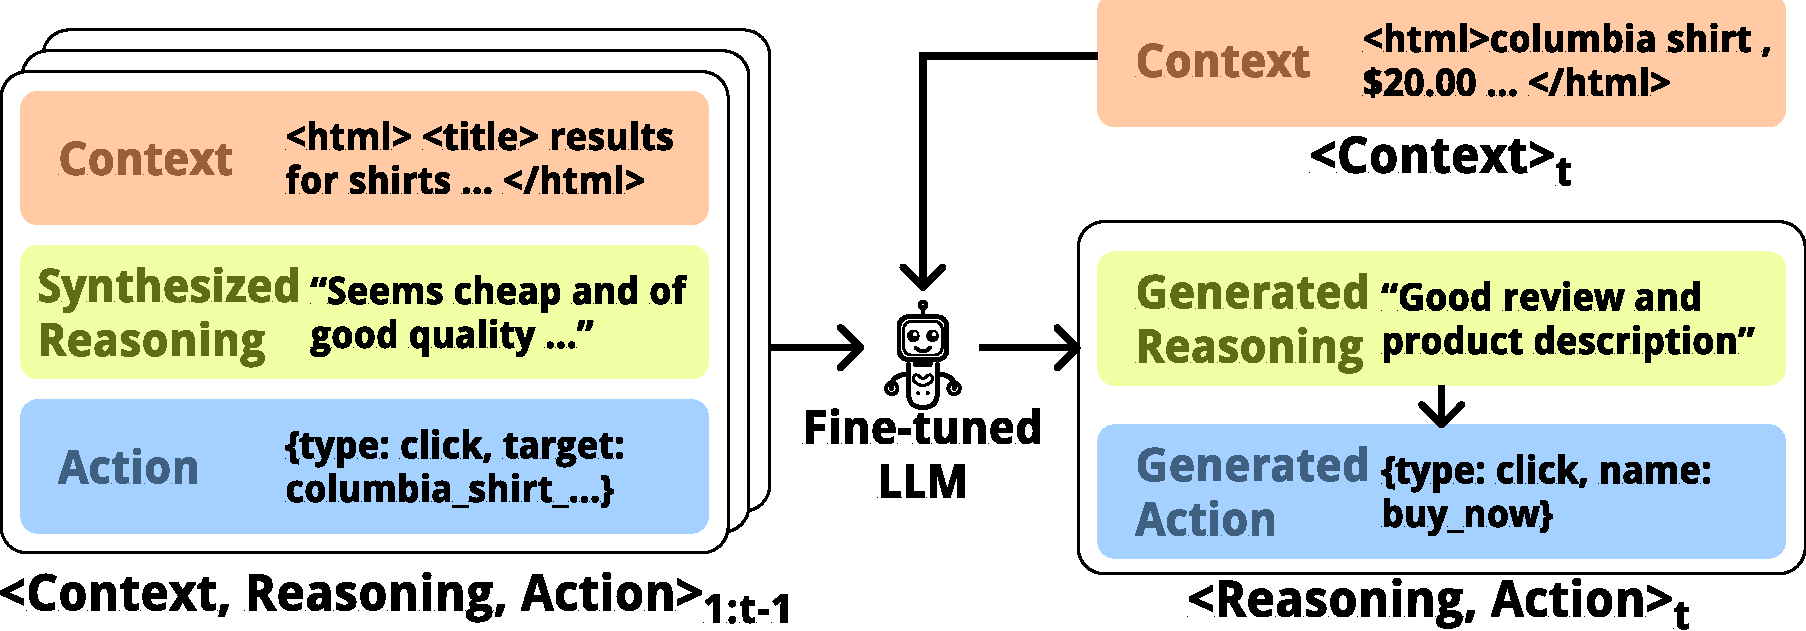
\includegraphics[width=\linewidth]{figures/teaser.pdf}
    \caption{Overview of the next action prediction task.}
  \end{figure}
\end{frame}

\begin{frame}{Dataset}
  \begin{outline}
    \1 Collected from a real-world online shopping platform.
    \1 31,865 sessions from 3,526 users
    \1 230,965 user actions
    \1 4,432 purchases, 27,433 terminations
  \end{outline}
\end{frame}

\begin{frame}{Context}
  \begin{outline}
    \1 \textbf{Context} (or the ``observation space'') is defined as the a ``simplified'' HTML-based representation of the current page.
    \1 JS and CSS are removed.
    \1 Important structural information (Table, List, etc.) is preserved.
    \1 LLM already understands the HTML format, no need to re-define ``button'' and ``input'' etc.
    \pause
    \1 Each interactable element is assigned a unique ``name'' (e.g. \code{product_form.add_to_cart})
  \end{outline}
\end{frame}
\begin{frame}{Action}
  \begin{outline}
    \1 \textbf{Action} is defined as the next raw browser action conducted by the user.
      \2 Generalizable to other domains beyond online shopping.
    \1 \code{click} (click on an element)
    \1 \code{type_and_submit} (type text and submit a form by hitting enter)
    \1 \code{terminate} (user ends the session by closing the browser window)
  \end{outline}
\end{frame}


\begin{frame}{Reasoning}
  \begin{outline}
    \1 \textbf{Reasoning} is defined as a natural language sentence that describes the reasoning behind an action.
      \2 \textit{``I want to find a comfortable piece of clothing, so I’m looking for options with high ratings.''}
    \1 Enhances the explainability of the model.
    \1 Not present in existing datasets.
  \end{outline}
  
\end{frame}

\begin{frame}{Rationale Synthesis}
  \begin{outline}
    \1 Reasoning traces are crucial for understanding users' action choices
    \1 Difficult to collect; thus, they are often not available in behavioral datasets.
    \1 Reasoning Synthesis Pipeline:
      \2 Record a real human customer's think-aloud shopping sessions as in-context learning examples.
      \2 Provide an LLM with the observation context and the corresponding action.
      \2 Use LLM to generate a free-text reasoning explaining the user's decision.
  \end{outline}  
\end{frame}

\begin{frame}{Finetuning LLMs}
  \begin{outline}
    \1 To enhance LLMs' accuracy in simulating human behavior, we finetune them on the task.
    \2 \textbf{Input:} ${\langle Context, Reasoning, Action\rangle}_{1:t-1}$ + $<Context>_t$ 
    \2 \textbf{Output:} $\langle Reasoning, Action\rangle _{t}$
    \1 Training:
      \2 Entire session is inputed as a whole.
      \2 Minimize the loss of the predicted action and reasoning tokens
    \1 Inference:
      \2 Input the context, past actions and corresponding reasoning.
      \2 Output the next action and reasoning.
  \end{outline}
\end{frame}

\section{Evaluation and Experiments}

\begin{frame}{Evaluation Metrics}
  \begin{outline}
    \1 Two tasks: 
    \1 Next Action Generation
      \2 Exact Match
      \2 Predicted action is only considered correct if both the action type (click, terminate, etc.) and the action attribute (the click target / the input text) match the ground truth.
      \pause
    \1 Shopping Outcome Prediction
      \2 Essentially predicting the last action based on the session history.
      \2 One of \code{click} on a \code{buy_now} button or \code{terminate} the session.
      \2 F1 score
  \end{outline}
\end{frame}

\begin{frame}{Models}
  \begin{outline}
    \1 Baseline Models:
      \2 Claude
      \2 Llama
      \2 Mistral
      \2 DeepSeek-R!
    \1 Fine-tuned Models:
      \2 Llama
      \2 Qwen
      \2 Mistral
  \end{outline}
\end{frame}

\begin{frame}{Results -- Accuracy \& F1}
  \begin{table}[t]
    \centering
    \begin{booktabs}{
      colspec = {X[l]cc},
      cells={m},
    }
    \toprule
    Model                         & { Action Gen. \\ (Acc.) }& {Outcome \\ (F1)} \\
    \midrule 
    {Llama 3.1 70B}       & 8.19\%              & 12.69\%            \\
    {Claude 3.5 Sonnet}& 9.72\%            & 15.91\%            \\
    {Claude 3.7 Sonnet}   & 9.34\%              & 12.81\%            \\
    {DeepSeek-R1}         & \textbf{11.86\%}             & \textbf{20.01\%}            \\
    Qwen2.5-7B           & 4.25\%              & 11.94\%      \\
    Mistral-7B-v0.3      & 4.25\%              & 11.27\%      \\
    Llama 3.2 3B         & 2.93\%              & 8.60\%       \\
    \midrule
    Qwen2.5-7B SFT                    & \textbf{17.26\% }            & 33.86\%            \\
    Mistral-7Bv0.3 SFT               & 15.84\%             & 30.12\%            \\
    Llama-3.2-3B SFT                  & 15.77\%             & \textbf{33.99\%}            \\
    \bottomrule
    \end{booktabs}
    \caption{Model performance.}
    \label{tab:results}
    \end{table}
\end{frame}

\begin{frame}{Results -- Distribution}
  \begin{figure}
    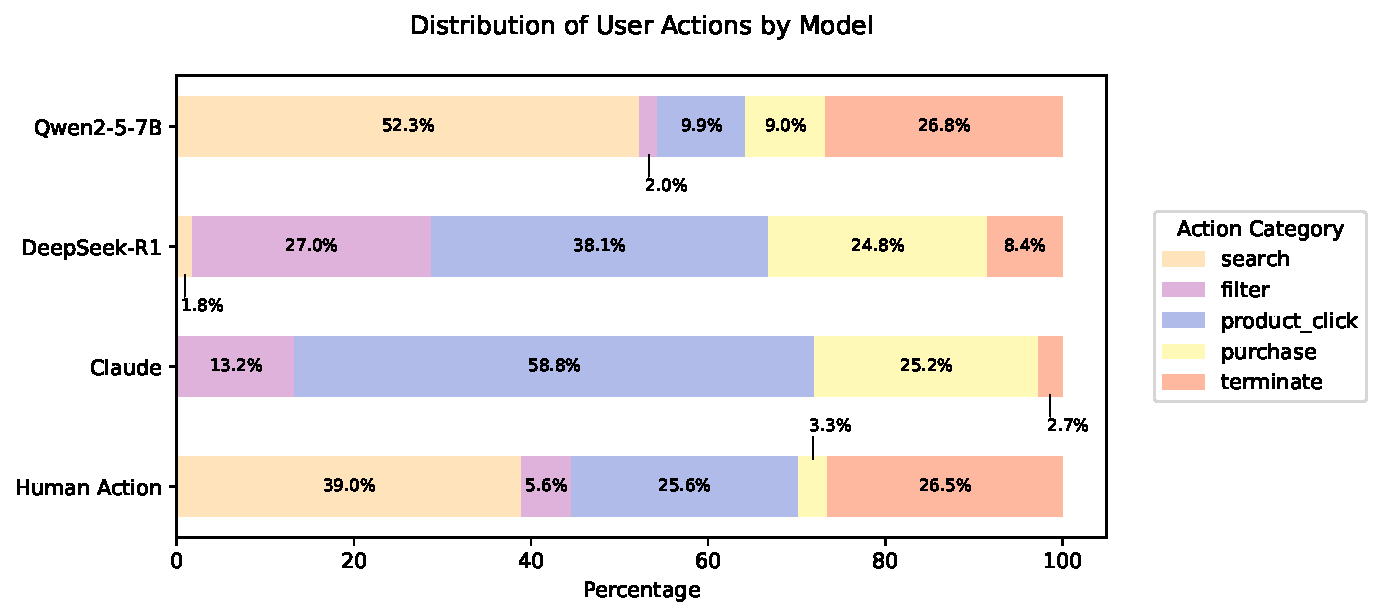
\includegraphics[width=\linewidth]{figures/action_distribution_below_labels.pdf}
    \caption{Distribution of the action types in the dataset.}
  \end{figure}
\end{frame}

\begin{frame}{Ablation Study}
  \begin{outline}
    \1 To evaluate the impact of training model with synthesized reasoning trace, we conduct an ablation study \textbf{to remove the reasoning trace} from the training data.

  \end{outline}
  \begin{table}[t]
    \centering
    \begin{booktabs}{
      colspec = {X[l]cc},
      cells={m},
      cell{3,5,7}{1}={r,font=\itshape},
    }
    \toprule
    Model                         & { Action Gen. \\ (Acc.) }& {Outcome \\ (F1)} \\
    \midrule 
    Qwen2.5-7B SFT                    & \textbf{17.26\% }            & 33.86\%            \\
    w/o reasoning                 & 16.67\%             & 26.92\%            \\
    Mistral-7Bv0.3 SFT               & 15.84\%             & 30.12\%            \\
    w/o reasoning                 & 14.17\%             & 17.99\%            \\
    Llama-3.2-3B SFT                  & 15.77\%             & \textbf{33.99\%}            \\
    w/o reasoning                 & 9.31\%              & 4.73\%             \\
    \bottomrule
    \end{booktabs}
    \caption{Ablation study result.}
    \label{tab:ablation}
    \end{table}
\end{frame}

\begin{frame}{Error Analysis}
  \begin{outline}
    \1 We analyze the errors made by the models: Claude and Qwen 2.5 7B.
    \1 Error types\footnote{Illegal actions generated by models are excluded from this analysis.}:
      \2 Didn't terminate
      \2 Didn't click
      \2 Didn't search
      \2 Searched wrong keyword
      \2 Clicked wrong button
  \end{outline}
\end{frame}

\begin{frame}{Error Analysis}
  \begin{figure}
    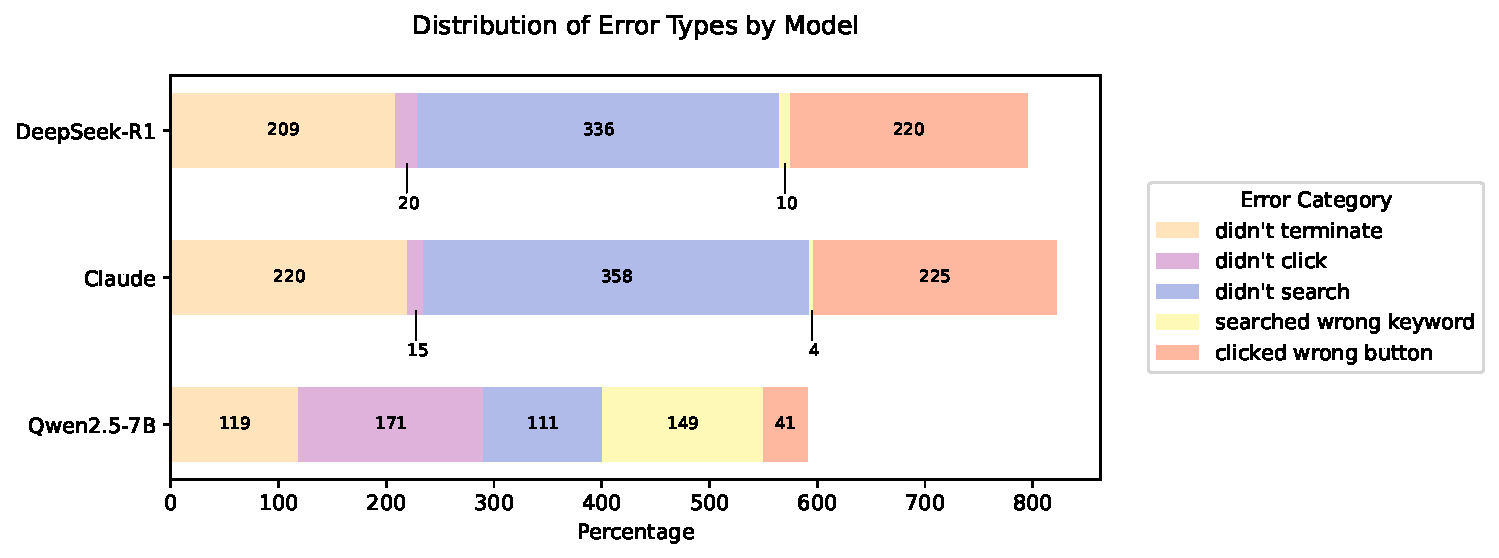
\includegraphics[width=\linewidth]{figures/error_analysis.pdf}
    \caption{Error analysis.}
  \end{figure}
\end{frame}

\section{Conclusion}

\begin{frame}{Conclusion}
  \begin{outline}
    \1 We present the first quantative, process-centric evaluation of LLMs for simulating human behavior in online shopping.
    \1 State-of-the-art models cannot simulate human behavior accurately, i.e. \textit{Prompting is not all-you-need!}
    \1 Fine-tuning with reasoning traces significantly improves the accuracy of LLMs in simulating human behavior.
  \end{outline}
\end{frame}

\begin{frame}[standout]
  Questions?
  [todo] add QR Code / final conclusions
\end{frame}


\end{document}


